\documentclass{article}
\usepackage{amsmath}
\usepackage[utf8]{inputenc}
\usepackage{mathtools}
\usepackage{tikz}
\usepackage[backend=biber]{biblatex}
\usepackage{titling}
\usepackage{titletoc}
\usepackage{graphicx}
\usepackage[document]{ragged2e}

\usepackage{amsmath}
\usepackage{amssymb}
\usepackage{amsthm}
\usepackage{mathtools}
\usepackage{array}
\usepackage{tikz}
\usepackage{hyperref}
\usepackage{enumitem}
\usepackage{stmaryrd}
\usepackage{subcaption}
\usepackage{titling}

%%%% Title page commands %%%
\newcommand\email[1]{
    \href{mailto:#1}{\url{#1}}
}

% Takes: name, affiliation & email
\newcommand\authorblock[3]{
    #1\\
    \small{#2}\\
    \small{\email{#3}}
}

\newcommand\keywords[1]{
    \vspace{5mm}\noindent
    \small{\textbf{\textit{Keywords ---}} #1}
}

%%% Short-hands %%%
\newcommand\NN{\mathbb{N}}
\newcommand\ZZ{\mathbb{Z}}
\newcommand\RR{\mathbb{R}}
\newcommand\CC{\mathbb{C}}

%%% Theorem environments %%%
\newtheorem{thm}{Theorem}
\newtheorem{lemma}{Lemma}
\newtheorem{prop}{Proposition}
\theoremstyle{definition}
\newtheorem{defn}{Definition}

\date{\today}

\addbibresource{newproposal.bib}

 \providecommand{\keywords}[1]
{
  \small
  \textbf{\textit{Keywords---}} #1
}



\title{Simulating the Water Molecule using the Spectrum by Quantum Walk Algorithm}


\begin{document}


\begin{titlepage}
    \newcommand{\HRule}{\rule{\linewidth}{0.5mm}}

	\center

	\HRule\\[0.4cm]

	{\huge\bfseries \thetitle\\[0.4cm]}

	\HRule\\[1.5cm]

	\begin{minipage}{0.45\textwidth}
		\begin{flushleft}
			\large
			\textit{Author}\\
            Floris van den Ende\\
            {\small Amsterdam University College}\\
            {\small\email{florisvdende@gmail.com}}
		\end{flushleft}
	\end{minipage}
	~
	\begin{minipage}{0.4\textwidth}
		\begin{flushright}
			\large
			\textit{Supervisor}\\
            Dhr. Dr. J.van Wezel\\
            {\small{Faculteit der Natuurwetenschappen en Informatica \& Qusoft}\\
            {\small{\url{j.vanwezel@uva.nl}}}}
		\end{flushright}
    \end{minipage}
    \\[1cm]
    \begin{minipage}[t]{0.45\textwidth}
		\begin{flushleft}
			\large
			\textit{Tutor}\\
            Dr. Forrest Bradbury\\
            {\small Amsterdam University College}\\
            {\small\email{f.bradbury@auc.nl}}
		\end{flushleft}
	\end{minipage}
	~
	\begin{minipage}[t]{0.4\textwidth}
		\begin{flushright}
			\large
			\textit{Daily Supervisor}\\
            Joris Kattemolle\\
            {\small Qusoft}\\
            {\small\email{j.j.kattemolle@uva.nl}}
		\end{flushright}
	\end{minipage}
    \vfill\vfill\vfill

    {\large
        Major: Sciences\\[0.5cm]
        \thedate

           }
           \vfill\vfill
    \includegraphics[width=0.2\textwidth]{{auc-logo.png}}\\[1cm]

	\vfill


\end{titlepage}



\abstract{This capstone will build towards understanding complex chemical reactions using quantum computing, by examining the efficiency of the Spectrum by Quantum Walk algorithm proposed by \textcite{poulin} applied to the water molecule. This algorithm will be implemented using Google's Cirq package and the ground state energy of the static water molecule will be retrieved. Ultimately, this capstone will compare the efficiency of aforementioned algorithm to several well-established other algorithms, where the conclusion of this comparison might be extrapolated to more complex chemical reactions. Quantum computing can help elucidate processes such as nitrogenase, where a greater understanding might lead to a severely reduced global energy output.}

\keywords{quantum computing, quantum walk, cirq, water molecule, quantum chemistry}

\section{Introduction}

Quantum computing is one of the most promising emerging scientific and technological fields of the past decades. The theoretical computational advantages of quantum computing allow for valuable applications in fields such as cryptography, chemistry and machine learning. However, quantum computing is no straightforward task: the fundamental issue is to perform high-fidelity operations on a coherent, scalable set of qubits \cite{malley}. Another fundamental objective is to manipulate the quantummechanical properties of your qubits as efficiently as possible, using algorithms. Peter Shor's prime factorization algorithm first showed the potential of quantum algorithms, and this research aims to find the most efficient algorithm for the ground state energy problem in chemistry \cite{shor}.


This problem is highly relevant, as three percent of the world's energy output is spent on making fertilizer \cite{reiher}. We currently rely on a highly outdated, energy-intensive process requiring very large amounts of natural gas. However, there exists an anaerobic bacteria performing a process serving the exact same function while requiring much less energy, utilizing nitrogen fixation with molecules such as FeMoCo. Traditional chemical analyses have not been able to give us an understanding on the details of this process, and as this molecule is highly complex, simulations using classical supercomputers are out of reach. \textcite{reiher} have shown that quantum computers are, even when taking in account the substantial decoherence and error of current gate computations, able to elucidate chemical processes such as nitrogen fixation in nitrogenase \cite{reiher}. Current research within quantum computing has not yet been able to provide significant insight into nitrogenase, and this study aims to build towards understanding more complex chemical reactions with quantum computers by examining the efficiency of a quantum walk ground-energy algorithm on the water molecule. If the scientific community succeeds in elucidating nitrogenase, new and more efficient processes of creating fertilizer may be developed, significantly reducing the global carbon footprint.


\section{Research Context}

The most fundamental property of a static molecule is the energy of the  molecule in its ground state. Before any other significant conclusions can be drawn about a molecule, the ground state energy must be known and accurately measured. If the field of quantum computing wishes to contribute to the understanding of chemical processes, it must succeed in efficiently retrieving the eigenvalues and eigenstates of the Hamiltonian operator of the molecule. The water molecule is simple enough for a classical computer to simulate and the ground state energy can be determined with the Hartree-Fock method, allowing this thesis to find the accuracy of the results of the algorithm \cite{smith}. The energy corresponding to the binding angle is portrayed in figure 1.

\begin{figure}[htbp]
    \centering
    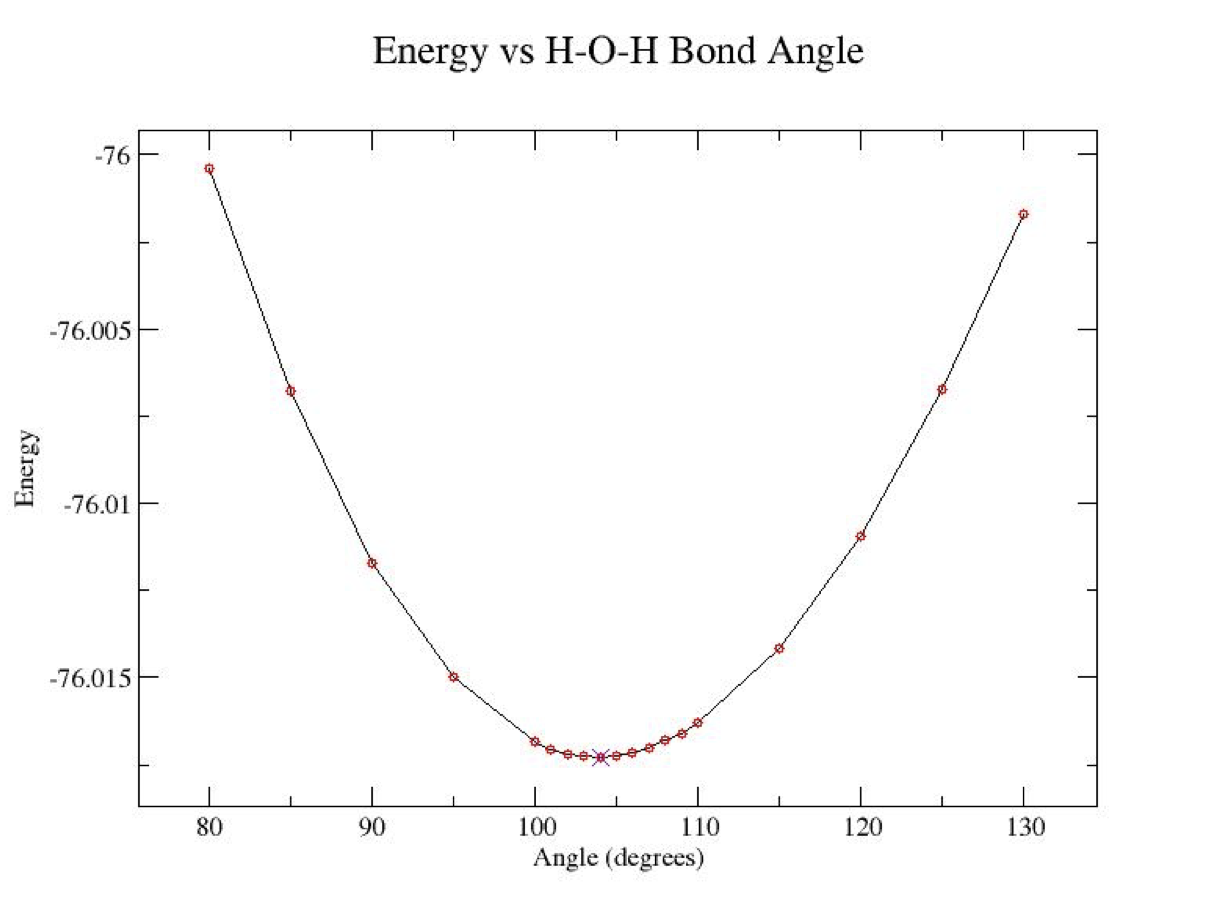
\includegraphics[scale=0.4]{h2oenergy.png}
    \caption{Energy of the $H_{2}O$ molecule over the molecular bond angle \cite{smith}.}
    \label{water}
\end{figure}

The second quantized Hamiltonian of the static water molecule generally is of the form \cite{bian}:

$$
H=\sum_{i, j=1}^{12} h_{i j} a_{i}^{\dagger} a_{j}+\frac{1}{2} \sum_{i, j, k, l=1}^{12} h_{i j k l} a_{i}^{\dagger} a_{j}^{\dagger} a_{k} a_{l},
$$

where $ a_{i}^{\dagger}$ and $a_{j}$ are the fermionic creation and annihilation operators and $ h $ is the respective interaction coefficient. In the ground state, we can assume that the two uppermost orbitals of the oxygen atom are unoccupied. In that case, 12 spin-orbitals have to be taken in consideration and the Hamiltonian is a sum over each one of these spin states.
\textcite{bian} reduce this Hamiltonian, using parity transformations and simplifications to the following form:

$$
H=\sum_{i=j}^{N} \alpha_{j} P_{j}
$$

Here, $\alpha_{j}$ is a function of the hydrogen-hydrogen bond length, and $ P_{j}$ is a multi-qubit Pauli operator, a tensor product of the four Pauli operators which are defined as the following \cite{malley}:


$$
X=\left(\begin{array}{cc}
0 & 1 \\
1 & 0
\end{array}\right), \quad \quad Y=\left(\begin{array}{cc}
0 & -i \\
i & 0
\end{array}\right), \quad \quad Z=\left(\begin{array}{cc}
1 & 0 \\
0 & -1
\end{array}\right),\quad \quad I=\left(\begin{array}{cc}
1 & 0 \\
0 & 1
\end{array}\right)
$$




An example of a multi-qubit Pauli operator would then be: $$ P = Z \otimes X.$$
The Hamiltonian consists of a sum of up to $N$ terms, where in this case $N = 2^4 = 16$, equal to the number of possible multi-qubit operators. Once the Hamiltonian is reduced, the ground energy can be derived from the Hamiltonian. There are several well-established algorithms. \textcite{bian} compare five methods for calculating the ground-state energy of the water molecule, namely:

\begin{itemize}
  \item \emph{Trotter Phase Estimation Algorithm}
  \\ This method uses Trotter-Suzuki decompositio(n to approximate  the propagating term $ e^{-i \alpha_{i} h_{i} t}$, and subsequently extracts the ground state energy from the phase. The Trotter PEA requires $\mathcal{O}(n)$ qubits to run and has a gate complexity of $\mathcal{O}(\frac{n^{5}}{(\epsilon / A)^{2}})$, where $n$ is the number of orbital basis functions, $A=\sum_{i=1}^{L}\left|\alpha_{i}\right|$ and $\epsilon$ is the desired accuracy of the energy.
  \item \emph{Direct Implementation of Hamiltonian in First Order}
  \\This method largely relies on the same principles as the Trotter PEA, but it employs a different unitary operator $U$. This Direct-PEA requires $\mathcal{O}(n)$ qubits to run and has a gate complexity of $\mathcal{O}(\frac{n^{5}}{(\epsilon / A)^{2}}).$
  \item \emph{Direct Implementation of Hamiltonian in Second Order}
  \\This method is the same as the First Order Direct-PEA, but it approximates $U$ to the second order instead. This variant of the Direct-PEA requires $\mathcal{O}(n)$ qubits to run and has a gate complexity of $\mathcal{O}(\frac{n^{5}}{(\epsilon / A)^{1.3}}).$
  \item \emph{Direct Measurement of Hamiltonian}
  \\This method translates the Hamiltonian directly into a quantum circuit and retrieves the ground energy by repeatedly measuring. Direct measurement requires $\mathcal{O}(n)$ qubits to run and has a gate complexity of $\mathcal{O}(n^{5}).$
  \item \emph{Variational Quantum Eigensolver}
  \\The VQE prepares a trial wave function and approximates the energy by iteratively retrieving the Pauli operator tensor products. This algorithm is often used on hybrid computers, as the the optimization algorithms required are much faster on a classical computer than a quantum computer. The VQE only requires $n$ qubits to run, and has a gate complexity of $\mathcal{O}(n^{2} d)$, where d is the number of iterations of entangling gates.

\end{itemize}

According to \textcite{bian}, it is evident that all five methods are viable options for solving the ground energy problem. There are however some major variations regarding gate complexity and qubit number. Second order Direct-PEA has the best gate complexity, but the VQE seems to be the most practical method for the near future, as it has decently efficient gate computations and, most importantly, requires the least amount of qubits.


The number of possible methods for the ground state problem are obviously not limited to the aforementioned five. \textcite{poulin} recently proposed another method named Spectrum by Quantum Walk, which bypasses the need to approximate the time-evolution operator, by initializing the quantum computer to an invariant subspace of the unitary operator. Doing so allows you to use any unitary operator which is a function of the Hamiltonian. \textcite{poulin} offer a specific unitary operator which, when initialized in the right bases, can be precisely implemented, avoiding any errors that might come with Trotter or Taylor approximations. Currently, no research has applied the Spectrum by Quantum Walk algorithm to the water molecule.
\section{Methodology}


The research process of this capstone will be composed of three main components. The first component consists of a literature review on the fundamentals on quantum computing, introducing standard conventions and treating concepts appearing frequently in later sections. To do so, several established texts such as \textcite{nielsen}, \textcite{steane} and \textcite{Divincenzo} will be synthesised. The second component expands on and provides context for the algorithm proposed by \textcite{poulin}, and it will also elucidate the relevant atomic structure of the water molecule in the form of a literature review. Furthermore, this part will also cover the implementation of the algorithm into a quantum circuit using Cirq \footnote{https://github.com/quantumlib/Cirq}, Google's open-source Python-based quantum computing package. The final part of this thesis will apply the quantum circuit of the algorithm to the specific Hamiltonian of the water molecule, retrieving the eigenstates of the Hamiltonian. Ultimately, this paper aims to develop an order of gate complexity as to compare the efficiency of the quantum walk algorithm to the five methods presented by \textcite{poulin}.

\newpage
\subsection{Table of contents of final thesis}

\begin{enumerate}
  \item Introduction
  \item Quantum Computation
  \begin{itemize}
    \item Why Quantum Computing?
    \item Gate Operations
    \item Quantum Circuits
    \item Quantum Algorithms
  \end{itemize}
  \item Spectrum by Quantum walk
  \begin{itemize}
    \item Overarching Principle
    \item Mathematical details
  \end{itemize}
  \item Quantum Circuit Implementation
  \item Application to the Water Molecule
  \begin{itemize}
    \item Quantum Chemistry
    \item Hamiltonian of the Water Molecule
  \end{itemize}
  \item Results
  \item Discussion
  \item Conclusion
\end{enumerate}

\subsection{Timeline}

\begin{table}[h]
\centering
\begin{tabular}{rll}
Before week &  & Tasks done  \\
\hline
7 & & Fully understand the algorithm and write chapter 2           \\
9 & Writing Update & Hand in chapter 2 and 3 and learn Cirq          \\
11 && Implement the algorithm to circuit, write chapter 4           \\
13 && Analyze the results, write chapter 5 and 6          \\
14 &Final thesis draft         & Write the Introduction and chapters 7 and 8         \\
17 &Final thesis         & Incorporate the feedback and finalize the thesis          \\

\end{tabular}
\end{table}

\nocite{reiher}
\nocite{nielsen}
\nocite{bian}

\printbibliography


\end{document}
